   
 
\documentclass[a4paper,10pt]{article}
\usepackage[utf8]{inputenc}
\usepackage[margin=25mm]{geometry}
\usepackage[italian]{babel}
\usepackage{amsmath}
\usepackage{amsthm}
\usepackage{amsfonts}
\usepackage{centernot}
\usepackage{multicol}
\usepackage{tikz}
\usepackage{listings}
\usepackage{courier}
\usepackage{MnSymbol}
\usetikzlibrary{patterns.meta}
\setlength{\parindent}{0em}
\newcommand{\reals}{\mathbb{R}}
\newcommand{\integers}{\mathbb{Z}}
\newcommand{\naturals}{\mathbb{N}}
\newcommand{\cnot}{\centernot}
\usepackage{graphicx}
\graphicspath{ {./images/} }

\definecolor{backcolour}{rgb}{0.95,0.95,0.92}
\lstdefinestyle{mystyle}{
    language=java,
    backgroundcolor=\color{backcolour},
    numberstyle=\tiny,
    basicstyle=\ttfamily\small,
    keywordstyle=\bfseries,
    breakatwhitespace=false,
    breaklines=true,
    captionpos=b,
    keepspaces=true,
    numbers=left,
    numbersep=5pt,
    showspaces=false,
    showstringspaces=false,
    showtabs=false,
    tabsize=2
}

\lstset{style=mystyle}

\begin{document}


\begin{center}
    \LARGE Giorno 6\smallskip

    \Large OOP: Ereditarietà multipla
\end{center}\smallskip

\section{Ereditarietà Multipla}
\subsection{Introduzione e motivazione}
Assumiamo di avere la seguente gerarchia di classi:
\begin{center} 
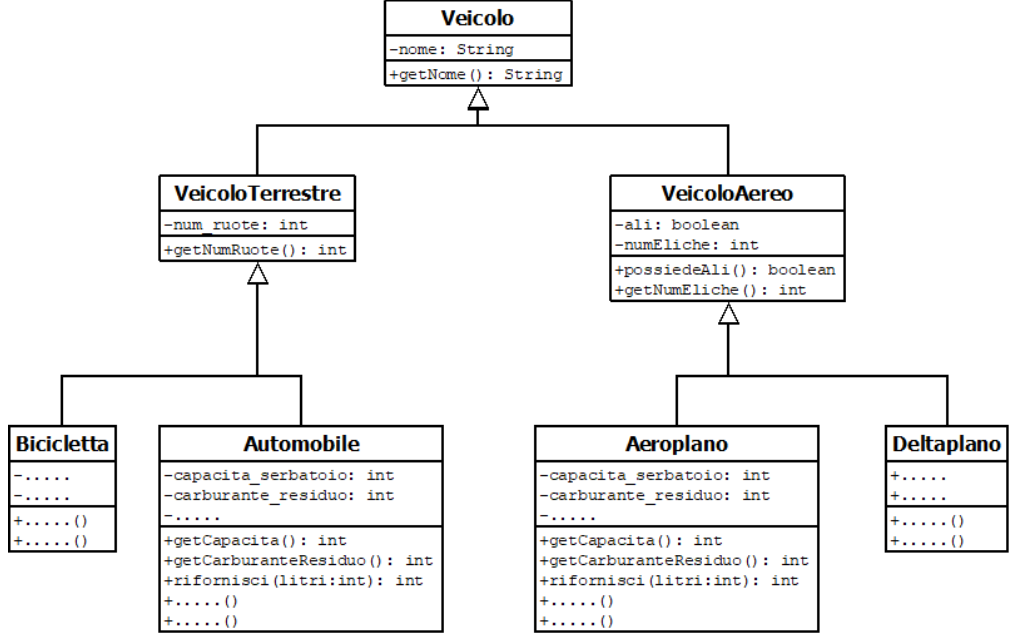
\includegraphics[scale=.5]{mult}
\end{center}

Le classi ``Automobile'' ed ``Aeroplano'' hanno in comune dei metodi  e degli attributi che non sono presenti nelle rispettive superclassi; dobbiamo implementare il codice due volte. In Java potremmo far sì che queste due classi implementino un'interfaccia comune, ma questo non risolverebbe (dobbiamo comunque scrivere il codice dei metodi due volte...)\smallskip

Vorremmo fare in modo che queste due classi estendano, oltre alle superclassi in figura, un'altra classe ``Rifornibile'', che fornisce i metodi e gli attributi in comune:

\begin{center} 
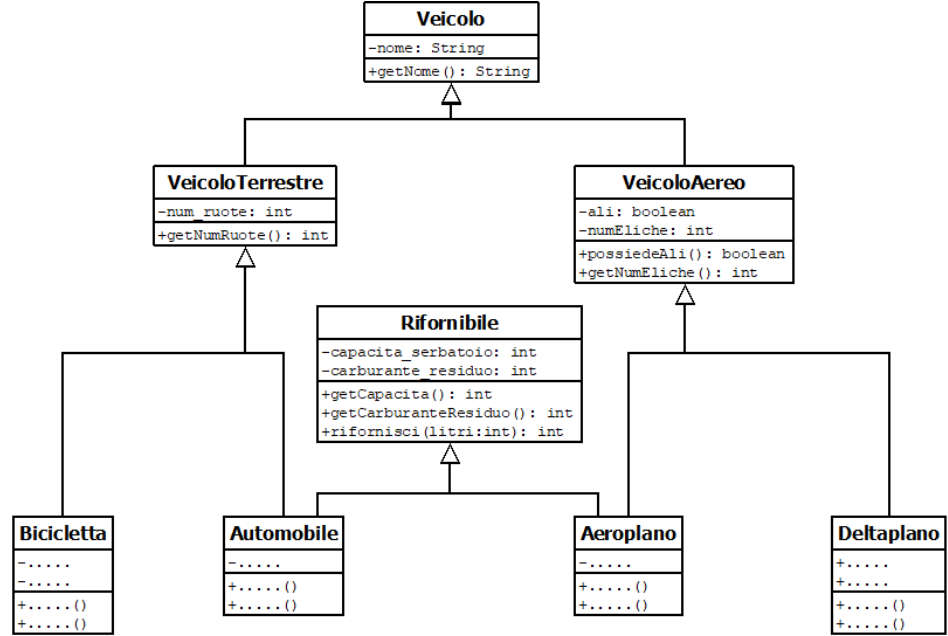
\includegraphics[scale=.5]{mult2}
\end{center}

Questo non si può fare in Java (ma in java 8 hanno aggiunto implementazioni standard nelle interfacce...)
\subsection{Problema dell'Ereditarietà Multipla}
\begin{itemize}
 \item Se entrambi i metodi estesi hanno un loro metodo con la stessa signature: quale si sceglie? 
 \item \textbf{Diamond problem}: Ereditare da due superclassi che possono \textbf{a loro volta avere una superclasse in comune} può portare a variabili d'istanza e metodi duplicati.
\end{itemize}
\subsection{Ereditarietà multipla in C++}
\subsubsection{Disambiguazione}
\begin{lstlisting}[language = c++]
#include <iostream>
using namespace std;
class A {
    int x = 10;
    public:
    A() { cout << "A" << endl; }
    void foo() { cout << "foo A" << endl; }
};
class B {
    int y = 20;
    public:
    B() { cout << "B" << endl; }
    void foo() { cout << "foo B" << endl; }
};
class C : public A, public B { // estende A e B
    int z = 30;
    public:
    C() { cout << "C" << endl; }
    void foo2() { cout << "foo2 C" << endl; }
};
\end{lstlisting}

\begin{lstlisting}[language=c++]
int main() {
    C c = C();
}
\end{lstlisting}

\begin{itemize}
 \item Si \textbf{noti} che non è stato scritto ``new'' davanti a \texttt{C()} 
 \item Eseguire questo codice stampa \texttt{A B C}, poiché creare un oggetto $C$ evoca i costruttori di $A$ e $B$, nell'ordine, prima di eseguire il proprio.
 \item A livello del \textbf{runtime di C++}, Il dispatch vector di $C$ è diviso in due parti: una con i metodi di $C$ ed $A$ (ossia, il dispatch vector ``come se ci fosse ereditarietà singola'') ed uno che punta ai metodi di $B$: questo ci permette di scegliere quale versione di \texttt{foo()} eseguire, usando questa sintassi:
 \begin{lstlisting}[language = c++]
c.A::foo()\end{lstlisting}
(vedi slide per schema -- Trattazione non estensiva, rivedere pezzettino di lezione se necessario)
 
\end{itemize}
\subsubsection{Diamond problem}\begin{multicols}{2}
                                
Se due classi $B$ e $C$ estendono una singola classe $A$, ed una classe $D$ estende $B$ e $C$, che succede se cerco di chiamare un metodo di $A$?

C++ pensa che ci sia da disambiguare tra due istanze del metodo: Il problema si scrivendo che le classi $B$ e $C$ estendono \textbf{virtual }$A$, invece di $A$.

In questo modo $A$ è generato una volta sola.\bigskip

\begin{center}
 
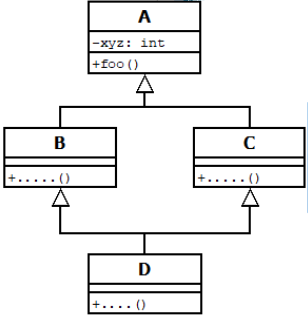
\includegraphics[scale = .6]{diamond}

\end{center}

\end{multicols}

\textbf{Esempio}

\begin{lstlisting}[language = c++]
#include <iostream>
using namespace std;
class A {
    public:
        int xyz = 10;
        A() { cout << "A" << endl; }
        void foo() { cout << "foo A" << endl; }
};
class B : public A { // da sostituire con "virtual public A"
    public:
        B() { cout << "B" << endl; }
};
class C : public A { // da sostituire con "virtual public A"
    public:
        C() { cout << "C" << endl; }
};
class D : public B, public C {
    public:
        D() { cout << "D" << endl; }
};
\end{lstlisting}

\begin{lstlisting}
int main() {
    D d = D();
}
\end{lstlisting}
Il programma stampa: \texttt{A B A C D}; il costruttore di $A$ è chiamato due volte, e se cerco di chiamare \texttt{d.foo()} ottengo un errore ``reques for member `foo' is ambiguous'', che propone come candidati i due metodi \texttt{foo} delle due istanze di $A$.\smallskip

\textbf{Nel runtime di C++}, la classe $D$ è costituita di due dispatch vectors:
\begin{itemize}
 \item Parte $A$, $B$, $D$ (cammino più a sinistra)
 \item Parte $A$, $C$ (cammino a destra)
\end{itemize}

E la tabella dell'oggetto $d$ è così strutturata
\begin{center}

 \begin{tabular}{|c|c|}
  \hline
  vtable A, B, D & $\to$ parte A, B, D\\
  \hline
  xyz & 10\\
  \hline
  vtable A, C & $\to$ parte A, C\\
  \hline
  xyz & 10\\
  \hline
 \end{tabular}

\end{center}


\textbf{Soluzione:} Se definisco $B$ e $C$ come \texttt{virtual}, il programma stampa \texttt{A B C D}, nessun problema. \smallskip

\textbf{Nel runtime di C++}, la classe $D$ è costituita di tre dispatch vectors:
\begin{itemize}
 \item Parte $B$, $D$ (cammino più a sinistra)
 \item Parte $C$
 \item Parte $A$ (da sola, perché è virtual)
\end{itemize}

E la tabella dell'oggetto $d$ è così strutturata
\begin{center}

 \begin{tabular}{|c|c|}
  \hline
  vtable B, D & $\to$ parte B, D\\
   \hline
  A & $\to$ ($\star$)\\
  \hline
  vtable C & $\to$ parte C\\
   \hline
  A & $\to$ ($\star$)\\
  \hline
  vtable A &($\star$) $\to$ parte A\\
  \hline
  xyz & 10\\
  \hline
 \end{tabular}

\end{center}

Come si può notare, per accedere alla vtable di $A$ c'è l'overhead di deferenziare un puntatore in più.

\paragraph{Perché virtual non è di default?} Per risparmiare tempo, proprio a causa di quella dereference in più: queste dereference potrebbero infatti concatenarsi ed accumularsi.
\newpage

\subsection{Interfacce multiple in Java}

In Java non c'è l'ereditarietà multipla, ma si possono definire più interfacce. 

\paragraph{Problema} Non si può usare lo sharing strutturale! Questo perché, se si implementano due interfacce, ci sono più membri con lo stesso indice (e.g. il primo elemento delle due interfacce ha indice zero)\smallskip

Si usa perciò una ``itable'', che contiene tutte le interfacce e i puntatori dai nomi dei metodi al loro codice.\smallskip

\begin{itemize}
 \item Vantaggi: La soluzione per la gestione edlle interfacce è trasparente al programmatore 
 \item Svantaggi: uso limitato dei meccanismi di ereditarietà
\end{itemize}

\subsubsection{Default methods}

Da java 8 si possono mettere implementazioni di default dei metodi nelle interfacce: questo ha introdotto di fatto l'ereditarietà multipla, con tutti i suoi problemi: \textbf{problema}, in caso di ambiguità il compilatore dà errore ed il programmatore deve modificare il codice dei metodi in conflitto (che schifo).\smallskip

Perché questa aggiunta? Gli sviluppatori Java hanno aggiunto le funzioni anonime, ed hanno esteso le collezioni per supportarle. \textbf{Problema}: non potevano aggiungere metodi alle interfacce se questi sarebbero risultati non implementati in tutti i programmi che usavano le collezioni, per retro compatibilità; perciò hanno aggiunto la possibilità di avere delle implementazioni di default.

\subsection{Ereditarietà multipla per linguaggi interpretati}
Nei linguaggi interpretati, la gestione dell'ereditarietà è basata su una visita del grafo che rappresenta la gerarchia. Visite diverse implicano scelte diverse in caso di ambiguità.

\subsubsection{Python}
Python linearizza il grafo (lo porta in \textit{method resolution order}) utilizzanodo l'algoritmo \textbf{C3}, che garantisce:

\begin{itemize}
 \item Determinismo
 \item Conservazione dell'ordinamento locale (se $c$ estende $c_1 \hdots c_n$ l'ordinamento prevede queste classi in quest'ordine)
 \item Monotonia ($c_1$ sottoclasse di $c_2 \implies $ $c_1$ viene prima di $c_2$)
\end{itemize}

L'ordine si può ottenere, in python, usando \texttt{CLASSE.mro()}\smallskip

Esistono gerarchie di classi non linearizzabili:

\begin{lstlisting}[language=python]
 class A(X, Y):
    pass
class B(Y, X):
    pass
\end{lstlisting}

($\implies$ errore a tempo di esecuzione.)


\subsection{Mixin}
Un mixin è un componente che può essere ``mescolato'' ad una classe esistente. Posso usarlo per aggiungere metodi \textbf{condivisi} a più classi, senza creare una superclasse. Se si considera l'esempio iniziale di automobile ed aeroplano, ``rifornibile'' potrebbe essere realizzato come Mixin; in questo modo non c'è bisogno, in questi contesti, di ricorrere all'ereditarietà multipla. \smallskip

Ad esempio, in \textbf{Dart}, si può modificare una classe con un mixin utilizzando \textbf{with}.


\end{document}
